\chapter{Construcción de la Interfaz de Consultas}
Después de haber seleccionado cuales serían los clasificadores que se utilizarían para realizar las predicciones en cada una de las áreas académicas, se debió tomar la decisión de cuál sería la mejor manera de presentar una interfaz de consultas, para que un usuario pudiera consultar cual sería el posible puntaje que obtendría un evaluado en cada una de las áreas académicas.

El primer aspecto a tener en cuenta era la interpretación de los clasificadores construidos. Weka permite guardar, en un archivo codificado, la estructura de un clasificador entrenado, para posteriormente utilizarlos con instancias de pruebas. Pero estos archivos codificados solo pueden ser cargados por las librerías de Weka. Es decir, que para poder utilizar los clasificadores creados, en la aplicación se debían utilizar estas librerías, por lo tanto el lenguaje base de la aplicación debía ser Java\footnote{\url{http://www.java.com}}.

El segundo aspecto que se tuvo en cuenta para la construcción de la interfaz, fue que analizando las vistas minables seleccionadas y realizando una intersección entre los atributos de los que estaba compuesta cada una, se tenía un total de 18 parámetros a preguntar. Esta cantidad de parámetros podrían ser fácilmente indagados en un formulación en HTML, además de que, una aplicación de escritorio en donde se tenga solo un formulario para obtener una respuesta es poco llamativo y se podría obtener un mayor acceso de usuarios si esta interfaz está construida sobre un entorno web.

Las ventajas que se obtienen con aplicaciones web son por ejemplo: que pueden ser accedidas siempre, sin importar en que dispositivos el usuario se encuentre: computador, laptop, tableta o teléfono inteligente. Se ejecutan sin importar el sistema operativo del usuario, no requieren instalación, entre otras.

Así, conociendo los 2 aspectos más importantes que debía cumplir la aplicación, se decidió utilizar la plataforma de programación J2EE de Java, la cual permite la creación de Servlets, los cuales son archivos de código Java que se ejecutan dentro de un contenedor de Servlets \cite{key-260}.

Los contenedores de Servlets capturan las peticiones que un usuario realiza sobre un servicio web y se encarga de procesar esta solicitud, enviársela al Servlet que procesa los datos y retorna una respuesta que de nuevo es procesa por el contenedor y entregada al navegador para que el usuario pueda visualizar los resultados de su petición.

Para la interfaz de navegación del usuario se utilizó la tecnología AJAX (Asynchronous JavaScript And XML). AJAX oficialmente es definido como: \begin{quote}“AJAX no es una tecnología en sí mismo. En realidad, se trata de varias tecnologías independientes que se unen de formas nuevas y sorprendentes.” \cite{key-270}.\end{quote}

AJAX permite que las consultas que se realizan desde una interfaz HTML hacia un servidor se realicen de manera asíncrona, evitando así la recarga constante de la página, cada vez que se desea consultar algo. Esto habilita al usuario a realizar diferentes tareas al tiempo, sin perder la posibilidad de continuar interactuando con la página.
\section{Arquitectura}
La arquitectura usada para la construcción de la aplicación, fue una arquitectura Cliente-Servidor. Del lado del cliente se tiene la capa de presentación que se carga por medio de un navegador web, esta presentación está construida usando HTML y una hoja de estilo CSS3.

La conexión con el servidor de Servlets se realiza a través de JavaScritp usando la tecnología AJAX y la librería JQuery\footnote{\url{http://jquery.com/}} para manipular el comportamiento de los componentes gráficos de la presentación, como el intercambio de div’s y estado de inhabilidad de los botones.

En el servidor se encuentra el Servlet PrediXaber, que se encarga de recibir los datos ingresados por el usuario y construir con ellos los archivos arff a ser ejecutados en los clasificadores. Estos archivos arff son creados agregando los datos de entrada a una plantilla predefinida, que tiene la estructura de datos que concuerda con cada uno de los clasificadores construidos.

Utilizando el archivo arff creado, se procede a cargar cada uno de los clasificadores usando las librerías de Weka, se ejecuta la clasificación por cada una de las áreas académicas y se construye una respuesta que es enviada, de nuevo, a través de AJAX. Esta respuesta se recibe y es cargada en la página HTML para que el usuario pueda observar los resultados de la consulta.

La figura \ref{fig:figura3} muestra gráficamente el diseño de la arquitectura de la aplicación.

\begin{figure}[!htb]
\begin{centering}
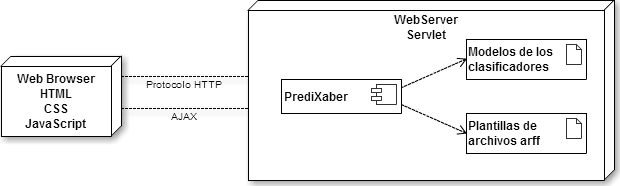
\includegraphics[scale=0.65]{package}
\par\end{centering}
\caption{Diseño arquitectónico de la aplicación.}
\label{fig:figura3}
\end{figure}
\section{Flujo de navegación}
El flujo de navegación normal que se debe seguir en la aplicación, es cargar la página principal donde se muestra el formulario con los campos requeridos para realizar la consulta. Después de  ingresar la información correspondiente al evaluado, se procede a enviar este formulario para que sea procesado en el servidor. La respuesta es retornada desde el servidor y desplegada en la pantalla para que el usuario pueda conocer los resultados de su consulta.

\begin{figure}[!htb]
\begin{centering}
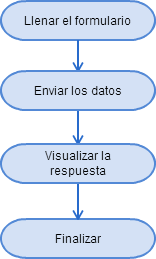
\includegraphics[scale=0.65]{Flowchart}
\par\end{centering}
\caption{Flujo normal de navegación que se sigue en la aplicación.}
\label{fig:figura4}
\end{figure}
\section{Codificación}
El proceso de codificación de la aplicación, se realizó utilizando los lenguajes programación Java y JavaScript, en Java se hizo uso de la librería Weka y en JavaScript de JQuery. Se utilizó HTML para definir los componentes de la página principal presentada al usuario y CSS3 para darle estilo a esos componentes.

En el ambiente de desarrollo se utilizó como IDE de desarrollo Eclipse\footnote{\url{http://www.eclipse.org}} y el contenedor de Servlets Tomcat\footnote{\url{http://tomcat.apache.org/}}.

Los parámetros que se envían al Servlet son procesados a través de un método POST para que la información sea enviada de manera codificada y no sea visible en la URL de la consulta. En el Servlet construido heredando la clase predefinida en java HttpServlet\footnote{\url{http://tomcat.apache.org/tomcat-7.0-doc/servletapi/javax/servlet/http/HttpServlet.html}} se construyó el método doPost() para procesar los datos recibidos y entregar una respuesta.

Dentro del Servlet la librería Weka se utilizó para la carga y ejecución de los clasificadores. Para cargar los archivos que contenían la información de los clasificadores se usó la clase SerializedClassifier, después de cargar la estructura, esta debía ser instanciada en un objeto del tipo Classifier para poder ejecutar el archivo arff. Se crea un objeto del tipo Instances que recibe como parámetro de construcción el BufferedReader que contiene el texto del archivo arff. Y por último, este objeto Instances es evaluado en el clasificador utilizando el método classifyInstance(), así se obtiene un valor para la clase a clasificar y este valor es retornado por medio del método doPost().

El código de la aplicación es sencillo, ya que solo se encarga de ejecutar las consultas usando los clasificadores anteriormente creados.
\section{Pruebas de usabilidad}
La usabilidad, en el software, se entiende como la facilidad que tiene un usuario de interactuar con la interfaz de las aplicaciones.

Los aspectos más importantes a evaluar en un diseño web son: curva de aprendizaje para el uso de la interfaz, eficacia de la interfaz, facilidad para memorizar, los errores que puede cometer el usuario y la satisfacción del usuario.

Para evaluar estos aspectos se hizo uso de la herramienta para evaluar usabilidad UsabilityHub\footnote{\url{https://usabilityhub.com/}}. Esta herramienta permita la creación de test que los usuarios pueden generar y compartir públicamente con las personas que ingresan a la página a responder estos test. 

Se hizo uso de 2 tipos de test. El test de Five Second, el cual le presenta al evaluador una imagen durante 5 segundos, después de ese tiempo realiza una pregunta que el evaluador debe responder. Y el test Click, el cual presenta una imagen acompañada de una pregunta en donde se le indica al evaluador que presione click en el lugar donde el cree que se ejecutaría cierta acción.

En el test de Five Second se presentó una imagen con el inicio de la página y se le pregunto al usuario sobre cual creía que era el objetivo de la página, después de leer la presentación. El 85\% de los encuestados, respondió que su finalidad era predecir resultados en la prueba saber 11\degree, el 15\% restantes, respondieron no tener clara la finalidad de la página.

En los test de Click se presentaron 3 imágenes, cada una con una pregunta sobre una acción a ejecutar. Las imágenes \ref{fig:figura5}, \ref{fig:figura6} y \ref{fig:figura7} muestra las preguntas realizadas y los resultados obtenidos.
\begin{figure}[!htb]
\begin{centering}
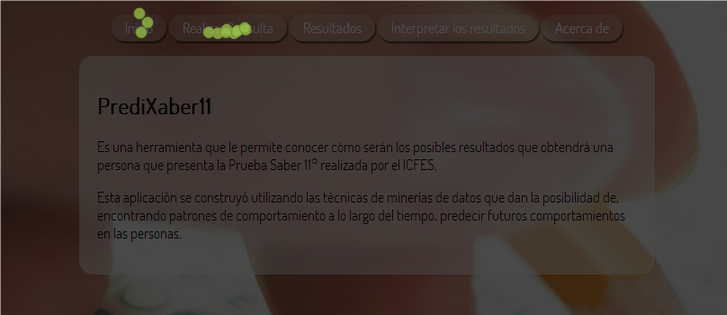
\includegraphics[scale=0.7]{realizarconsultatest2}
\par\end{centering}
\caption{Acción: Mira las opciones en los links y selecciona aquella que creas que te permitirá ejecutar una consulta.}
\label{fig:figura5}
\end{figure}
\begin{figure}[!htb]
\begin{centering}
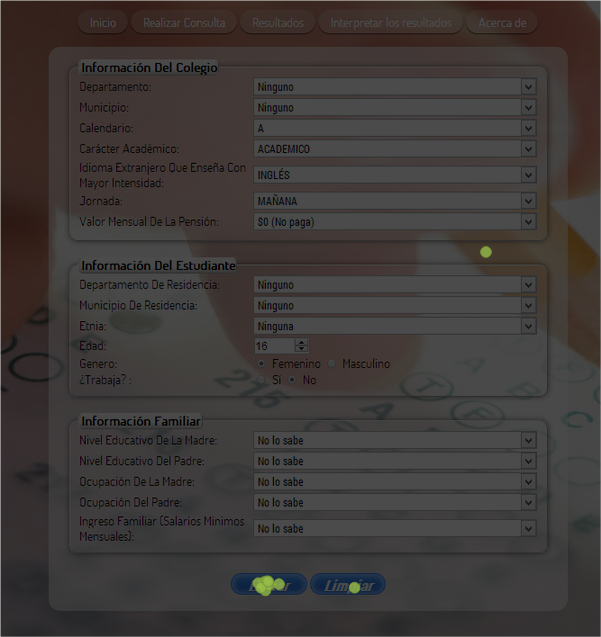
\includegraphics[scale=0.6]{enviarformulariotest}
\par\end{centering}
\caption{Acción: Donde harías click para enviar el formulario y recibir una respuesta.}
\label{fig:figura6}
\end{figure}
\begin{figure}[!htb]
\begin{centering}
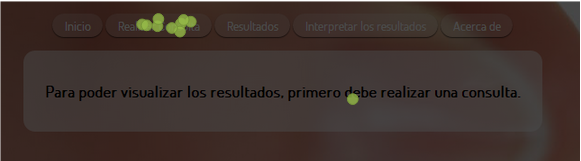
\includegraphics[scale=0.6]{realizarconsultatest}
\par\end{centering}
\caption{Acción: Donde harías click después de leer el mensaje.}
\label{fig:figura7}
\end{figure}
\section{Pruebas de código}
Para verificar la funcionalidad del código se generaron pruebas unitarias utilizando 2 frameworks diferentes pero conectables. Uno para evaluar que el flujo de navegación dentro de la aplicación retorne los resultados esperados y otro para evaluar que los métodos construidos dentro del Servlet funcionen correctamente al procesar la información recibida.
Para construir las pruebas del flujo de navegación se utilizó el framework de automatización de pruebas Selenium\footnote{\url{http://docs.seleniumhq.org/}}. Selenium permite grabar y reproducir pruebas a partir de un plugin que puede ser instalado en el navegador Firefox\footnote{\url{http://www.mozilla.org/en-US/firefox/new/}}. Con este plugin, el usuario inicia una grabación de pasos a seguir dentro del aplicativo web, entre cada paso ejecutado, el usuario puede agregar verificaciones de la respuesta o las respuesta esperadas al ejecutar ese paso.
Selenium también permite la ejecución de estas grabaciones, así cada vez que se desee verificar si los resultados esperados de una secuencia de pasos están siendo correctamente procesados, se ejecuta el script creado con anterioridad y se verifica este comportamiento.
Los scripts creados por Selenium pueden ser exportados a diferentes lenguajes de programación para ser ejecutados por otros frameworks de pruebas. Para el caso del presente trabajo, se decidió exportar el script creado al lenguaje de programación Java utilizando el framework de pruebas JUnit\footnote{\url{http://junit.org/}}.
Con JUnit también se construyeron tests para evaluar el comportamiento de los métodos definidos en el Servlet utilizado en el servidor para procesar las consultas del usuario. Se crearon 16 métodos de test en total que permiten verificar tanto el comportamiento de la interfaz de usuario y del código generado dentro de las clases.
\section{Pruebas de confiabilidad}
En esta prueba se quería comprobar la calidad de las predicciones realizadas por los clasificadores. Pero no individualmente, como ya se realizó, sino en conjunto ejecutando la solicitud al Servlet que realiza el procesamiento de los datos.

Para ejecutar esta prueba se utilizaron 100.000 registros de las bases de datos del año 2012, la cual ya se advirtió que no fue utilizada en la construcción de los clasificadores. Se creó un script en Python con el cual se ejecutaron las solicitudes al Servlet. A cada registro se le aplico la transformación de datos correspondiente.

Al recibir la respuesta de la solicitud se comparaban los resultados de las áreas académicas para encontrar en cuantas se realizaba correctamente la predicción.

La tabla \ref{tab:cuadro39} muestra los resultados de cuantas áreas académicas coincidieron. El total de áreas académicas en las que es evaluada una persona son 9, 8 de núcleo común y 1 de elección del evaluado.

\begin{table}[!Hhtb]
\centering
\begin{tabular}{|p{6.5cm}|p{6.5cm}|}
\hline
	\rowcolor[gray]{0.9} 
	\textbf{Cantidad de coincidencias} &
	\textbf{Cantidad de registros} 
	\\
\hline
9 & 98\\
\hline
8 & 881\\
\hline
7 & 3840\\
\hline
6 & 10116\\
\hline
5 & 17952\\
\hline
4 & 22166\\
\hline
3 & 20713\\
\hline
2 & 14598\\
\hline
1 & 8602\\
\hline
0 & 1034\\
\hline
\end{tabular}
\caption{Resultados de la prueba de confiabilidad realizada a la aplicación.}
\label{tab:cuadro39}
\end{table}
Se puede observar que cerca del 33\% de los registros evaluados (32.887) tienen al menos 5 coincidencias, que son más de la mitad de los puntajes a predecir. Se percibe que al momento de realizar consultas en conjunto sobre los clasificadores se pierde la calidad que estos mostraban de manera individual. Pero también se puede observar que las predicciones se comportan como una función gaussiana en  donde la mayoría de los resultados están agrupados en predicciones con el 50\% de confianza.